%\documentclass[10pt,a4paper]{article}
%\date{10318221}
%\author{Author: Sinead Hales}
%\usepackage[latin1]{inputenc}
%\usepackage{amsmath}
%\usepackage{amsfonts}
%\usepackage{amssymb}
%\usepackage{sectsty}
%\sectionfont{\normalsize}
%\usepackage[normalem]{ulem}

%\usepackage{multicol} 

%\usepackage{graphicx}

%\usepackage[top=1cm, bottom=2cm, left=2cm, right=2cm]{geometry} 
%\newcommand{\degree}{\ensuremath{^\circ}}
%\pagestyle{empty} 

\section{Evidence for CP-Violation in relation to cosmological models and detection via natural particle accelerators}
%\begin{document}
%\maketitle
%~\\

\subsection{Justification of the hot big bang model}

Consider our observable universe and it's contents, from scales to clusters of galaxies to the dust particles in between them, there appears to be a clear matter dominance over anti-matter, an asymmetry between the two. However from this asymmetry a contraction arise from the early big bang theory. One of the  explanation for this discrepancy is CP violation, the combination of the C, Charge Conjugation, and P, Parity operators. It is throughout this chapter that CP violations involvement with the matter dominance in the early universe and its applications to cosmology will be investigated. \\
\par The hot big bang model is one of the most widely accepted theory for the origin of our universe among the scientific community due to its empirical merits \cite{1}\cite{10}, however a naive or simplistic model is insufficient to explain the matter anti-matter asymmetry and it could be tempting to disregard this hypothesis. The model hypothesizes that the universe as we know it was born in an explosion of tremendous proportions and despite the mentioned inconsistencies, today there exist three main observations supporting this model.\cite{10} \\
\begin{itemize}
\item The Hubble expansion. \\ The concept of the expanding universe is one that the distance between any two point changes over time, the space itself expands rather than the objects themselves away once one another. A consequences of this effect is that, as light travels through this expanding space, its wavelength is also stretched. Consider the optical component of the electromagnetic spectrum, red light has a longer wavelength than blue, as the fabric of the universe expands, as does the wavelength of the light, hence light from distant objects appears more red, this process is known as red-shifting and the longer light travels through expanding space, the more redshifting it experiences. \cite{1} \cite{10}
Therefore, since light travels at a fixed speed, the big bang theory tells us that the redshift we observe for light from a distant object should be related to the distance to that object. \cite{11} \cite{10}
\item The cosmic microwave background. \\ The CMB was discovered in 1965 by Arno Penzias and Robert Wilson from Bell Labs. They were working with a microwave receiver on a radio telescope, but were getting a low frequency noise from every direction they pointed the receiver. They concluded that radiation was emanating from all directions in our observable locality of the universe.\cite{10} This was the first evidence for the CMB. \par Another interesting aspect of the CMB is a distribution of wavelengths in the centimeter and millimeter wavelengths that is characteristic of black body radiation at 2.7 K. A black body radiator is an idealized object that absorbs and emits all wavelengths of radiation, the extent of absorption and emission of a given wavelength depending on the blackbody's temperature. The Big Bang model predicts that at high temperature the universe is filled with a plasma, a blackbody radiator. This would occur as a result of an ambient temperature of about 3000K, at which hydrogen can only exist as a plasma.
As the universe continued to expand the plasma began to cool, it eventually reached the temperature where electrons were able to combine with nuclei to form neutral atoms.\cite{10} \cite{11} Before this recombination epoch, the Universe would have been opaque due to the free electrons causing photons to scatter. However, when the free electrons were absorbed to form neutral atoms, the Universe suddenly became transparent, this is afterglow is what we observe with the cosmic microwave background.
\item The relative primordial abundances of light elements (Helium 3 and 4, Deuterium, Lithium). \\ To begin with, it was estimated that only a small amount of matter found in the Universe should consist of helium if stellar nuclear reactions were its only source of production, however, due to advances in spectroscopy, physicists have successfully estimated that up to 25\% of the observable mass in the universe is helium.This value is too large to be explained by stellar fusion. \cite{1} \cite{10}  The abundance of lighter nuclei such as Li is also difficult to explain by stellar nucleosynthesis; however, the Big Bang model theorizes that the very early Universe was too energetic for matter and so all matter was fully ionized and dissociated. \cite{1}
\par After a short time after Big Bang itself, the temperature of the Universe rapidly cooled from an estimated value of $ 10^{32}$ Kelvin to approximately $10^{9}$ Kelvin. It was at this temperature, nucleosynthesis could begin. In a short time interval, protons and neutrons collided to produce elements such as deuterium, which is unable to be formed inside stellar cores because unlike helium, deuterium is a very fragile element. It gets destroyed at $10^{6} K$, which is below the temperature in a stellar core, which is on the order of $10^{6}-10^{8}$ Kelvin. \cite{10}
\end{itemize}
It is for these reasons that this theory is used for a framework for other predictions regarding our universe. One such prediction is that at the beginning there was once an absence of matter from the universe, only energy in the form of photons. As the universe expanded, another prediction obtained from the big bang, it cooled and hence became less energetic and turbulent, and matter was able to form through the process: \cite{5} 
\begin{equation}
\gamma + \gamma \ \rightarrow p+ \bar{p}.
\end{equation}
Where $ \gamma $ represents the photon, $p$ and $\bar{p}$ represents the particle and anti-particle respectively. Or in the language of Feynman diagrams\cref{fym}: 
\begin{figure}[hbt!]\label{fym}
\begin{center}
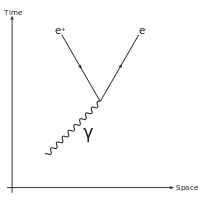
\includegraphics[width=0.451\textwidth]{figs/p.png}
\caption{Feynman diagram showing pair production from gamma ray photons}
\end{center}
\end{figure}
From looking at this interaction equal amounts of particles and anti-particle are produced and that if one were to consider these conditions alone it appears as though there should be a symmetry between matter and anti-matter. However, it is matter not anti-matter but matter that we observe out to distances of 10Mpc \cite{1} and there exists strong evidence that this is applicable to the universe as a whole. The evidence to support this lies in the fact that there are no large localised gamma ray sources that appear to not have a source, i.e. a diffuse background. In conclusion, there exists a contradiction between the simple formulation of the big bang model and the small ratio of anti-matter to matter, currently estimated at approximately $10^{-4}$ \cite{13}\cite{5}
~\\

\ %begin{center}
\subsection{Baryogenesis and Leptogenesis}
%\end{center}

The problem of the baryon asymmetry of the universe is a classic problem of particle cosmology, studies in particle physics has taught us that matter and antimatter behave essentially identically. However, cosmology teaches us that the early universe was an extremely hot, and hence energetic, environment in which one would expect equal numbers of baryons and anti baryons to be copiously produced, as described above.\cite{13} \cite{5} This early state of the universe stands in direct contradiction to what is observed in the universe today. Astronomical surveys and mission have shown that our universe contains no appreciable quantity of primordial antimatter. In addition, the theory of primordial nucleosynthesis allows accurate predictions of the cosmological abundances of all the light elements, while the only constraint begin that\cite{5}: 
\begin{equation}
2.6\cdot10^{-10} < \eta \equiv \frac{n_{b}}{n_{bar{b}}} < 6.2\cdot10^{-10},
\end{equation}
Where: 
\begin{itemize}
\item $\eta$ is the baryon asymmetry.
\item $n_{b}/ n_{bar{b}}$ is the number density of baryons/anti-baryons.
\item $s$ is the entropy density.
\end{itemize}
This as been calculated from precise measurements of the relative heights of the first two microwave background acoustic peaks by the WMAP satellite \cite{14} The baryon asymmetry can be also be expressed as:
\begin{equation}
0.015(0.011) < \Omega_{B}h^{2} < 0.026(0.038),
\end{equation}
Where: 
\begin{itemize}
\item $\Omega_{B}$ is the proportional critical density in baryons.
\item $h$ h parametrizes the present value of the Hubble parameter $(h = \frac{H_{0}}{100(KmMpc^{-1}sec^{-1})})$
\end{itemize}
As cosmic inflation occurred the universe cooled and hence the number of nucleons and anti-nucleons decreases\cite {1}, so long as the annihilation rate $\Gamma_{ann} \simeq n_{b} \left \langle {\sigma_{a}v} \right \rangle$ is larger than the expansion rate of the universe, where $\left \langle {\sigma_{a}v} \right \rangle$ is the averaged annihilation cross section. As the annihilations freeze out the anti-nucleons, being so rare, they cannot annihilate any longer. Therefore the ratios of baryons and anti-baryons becomes: \cite{1} \cite{14} \cite{11}
\begin{equation} \labe{eta}
\frac{n_{b}}{n_{\gamma}} \simeq \frac{n_{bar{b}}}{n_{\gamma}} \simeq 10^{-18},
\end{equation}
which is much smaller than the required value for nucleosynthesis to occur. An initial asymmetry could thought to be imposed as an initial condition rather than an afterward mechanism, however this would violate any naturalness principle . The next section the Sakharov Criteria which must be satisfied by any particle physics theory through which a baryon asymmetry is produced[\cite{5}\cite{13}].

\subsection{Conditions for baryogenesis}
Sakharov conditions for Baryogenesis\cite{5}, he described three processes of nature that were required for baryogenesis to occur. All of these ingredients are compatible the Standard Model. Whether or not a single mechanism can combine all of them to provide the baryon-dominated universe we see today is an open question \cite{5}.
\begin{itemize}
\item At least one B-number violating process.
\item C and CP violation.
\item Interactions outside of thermal equilibrium.
\end{itemize}
\subsection{B-number violation}
The Standard Model Lagrangian conserves B classically, but there is a global anomalies under which B- conservation could be violated. The canonical example is the sphaleron process. In electroweak gauge theory, the vacuum state is infinitely degenerate, and the different sub-states are separated by energy barriers[cite]. Through a quantum tunneling process, the system can move to a different vacuum sub-state which has nonzero baryon number.\cite{13}\cite{5} The sphaleron process is considered to be non-perturbative, so it is not possible to draw a true Feynman diagram for illustrate the process.
\par It is a static solution to the electroweak field equations of the Standard Model and geometrically, a sphaleron is simply a saddle point of the electroweak potential energy\cite{8}\cite{13}. In the standard model, processes violating baryon number convert three baryons to three anti-leptons, and related processes. This violates conservation of baryon number and lepton number, but the difference B-L is conserved. A sphaleron may convert baryons to anti-leptons and anti-baryons to leptons, and hence a quark may be converted to 2 anti-quarks and an anti-lepton, and vise versa.\cite{5}. While it cannot be shown in the form of a Feynman diagram, due to its non-perturbative nature, \cref{BL} shows an example of exchanging three leptons, one from each generation( electron, muon, tau), for nine quarks, three within each generation, and one of each color per generation. L and B are not conserved individually though the quantum number B - L is, consider the example\cite{13}:
\begin{equation}
\Delta L = \Delta B = \pm3 
\end{equation}
\begin{equation}
\Delta B - \Delta L = 0
\end{equation}
Essentially this process generates a baryon excess out of a lepton excess. \cite{5}
\begin{figure}[hbt!] \label{BL}
\begin{center}
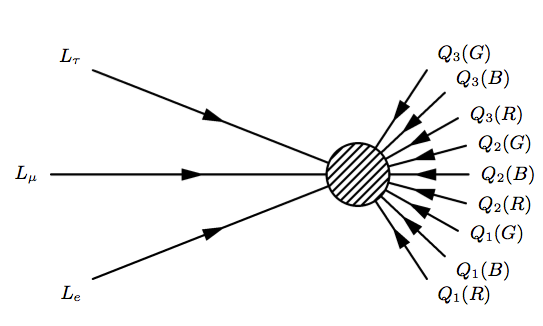
\includegraphics[width=0.451\textwidth]{figs/bl.png}
\caption{The incoming quantum numbers are L = 3 and B = 0. The outgoing quantum numbers are L = 0 and B = -3.}
\end{center}
\end{figure}
\subsection{Interactions outside of thermal equilibrium}
Even with CP-violation working in favor of baryogenesis, there are thermodynamic considerations. The energy difference between a particle and its corresponding antiparticle is \cite{5}:
\begin{equation}
\Delta E = m_{matter} + m_{matter} = 0
%\label{}
\end{equation}
At thermal equilibrium, the Boltzmann distribution dictates that there should be equal amounts of matter and antimatter. Other processes will turn any baryon asymmetry back into even numbers of baryons and anti-baryons. Thus, any baryogenesis must happen under conditions outside of thermal equilibrium.[cite] Once baryogenesis occurs, the universe returns to thermal equilibrium, this implies the conditions then must have changed such that the generated asymmetry cannot be reversed.\cite{5} \cite{13}
\par There is a natural setting for interactions outside of thermal equilibrium in the Standard Model. Consider the spontaneous electroweak symmetry breaking that happens during the electroweak phase transition  which is relevant for temperatures, $ T \sim 100 GeV $. An analogy for this phase transition mechanic is like bubbles of steam forming inside boiling water. The inside of the bubbles, where the symmetry has broken is at thermal equilibrium with its surroundings, as are the outside of the bubbles. For the boundary this is not the case. On the inter-phase between the two phases, all interactions occur outside of the equilibrium. As the bubbles expand to cover all space and the universe cools, the results of whatever happened on the boundaries become frozen in.\cite{5}\\
There are few possible mechanics to further explain this process.
\subsubsection{Electroweak phase transition}
his mechanism involves the three examples of the Sakharov conditions in the Standard Model above. During the electroweak phase transition, baryon-generating processes, the above mentioned sphaleron process, which took place at the inter-phase. Due to CP-violation, baryogenesis dominated over the conjugate process. After the transition ended, the temperature fell below the sphaleron mass. The baryon excess was therefore frozen in \cite{5} Current theoretical calculations result in a much lower value of $\eta$, as shown above see Eqn.(\ref{eta}), than experiment. In particular, CP-violation in the quark sector may not be enough to explain the large asymmetry. 
It is thought that the amount of CP actually observable, and/or the branching ratio of the decay mode is not of high enough significance to explain the large asymmetry between matter and anti-matter.
\subsubsection {Leptogenesis}
A large lepton excess is generated through a currently unknown mechanism, and then B - L conserving processes turn this into a baryon excess directly, see \cref{BL} fig.1. CP-violation in leptogenesis becomes effective CP-violation in baryogenesis. This mechanism is more attractive because CP-violation in the lepton sector is not nearly as constrained, mainly due to the fact that measuring it is much more experimentally challenging. This mechanism turns the mystery of baryogenesis into the complementary one of leptogenesis. \cite{5}
\subsection{C- and CP-Violations.}
Baryon number alone is not sufficient to account for the matter anti-matter symmetry, if the symmetry of the universe is charge conjugation [C], then is this quantity is conserved then all B-number violation reactions: \cite{5}
\begin{equation}
X \rightarrow Y + B
\end{equation}
has the same width as the charge conjugation reaction. The quantities X and Y have a baryon number of zero, and B is a non-zero excess baryons. The conjugation reaction is as follows: 
\begin{equation}
\Gamma (X \rightarrow Y + B) = \Gamma (\bar{X} \rightarrow \bar{Y} + \bar{B})
\end{equation}
Since both of the process happen as the same rate, over long time intervals the B-number is conserved. 
This justifies that C-Violation is a Sakharov conditions\cite{5}\\
In addition to this, next consider a hypothetical process that violates B-number, $X \rightarrow q_{L}q_{L}$, which results in the creation of left-handed baryons. This then occurs at the same rate as the CP conjugate process, $X \rightarrow q_{R}q_{R}$ and hence: 
\begin{equation}
\Gamma (X \rightarrow q_{L}q_{L}) + \Gamma(X \rightarrow  q_{R}q_{R}) = \Gamma (\bar{X} \rightarrow \bar{q_{L}} \bar{q_{L}}) + \Gamma(\bar{X} \rightarrow  \bar{q_{R}} \bar{q_{R}})
\end{equation}
In conclusion, the C-conjugate reactions have a different width, but the sum of the two will still preserve baryon number Thus, CP needs to be violated as well, so that the rate of baryogenesis exceeds that of anti-baryogenesis. With C- and CP-violation, the rate of $B-production$ can exceed that of $\bar{B}-production.$\cite{5} \cite{13}
\begin{center}
\section{Searching for evidence of CP in the diffuse gamma ray sky.}
\end{center}
\subsection {Introduction}

Magnetic fields in various astrophysical settings may in fact be helical and, in the cosmological context, may provide a measure of primordial CP violation during baryogenesis.\cite{2}\\
It is a safe assumption to make; that magnetic fields pervade all astronomical objects \cite{2} \cite{3}, expanding on this; there is strong theoretical evidence, predicted by current cosmological models, to support the idea that a weak magnetic filed pervades the entire universe itself. Motivated by this idea of a pervading cosmological magnetic field with non-trivial helicity(in cosmology, a number of scenarios predict the creation of a primordial field with non-zero helicity \cite{2}), a CP odd statistic, defined by Q, could be, theoretically evaluated be using gamma ray ray data from TeV blazars observed by Fermi satellite's instrument LAT \cite{9}. \\
Before an in-depth analysis can be made, foundations must first be laid by explaining certain concepts.
\begin{itemize}
\item {Helicity.} \\
By definition it is the projection of a particle's spin onto the direction of its momentum as the projection of the orbital angular momentum is zero along the linear momentum. \cite{4} Helical magnetic fields can be said to possess the property of a non-vanishing component in the direction of the current, $
B(\nabla \wedge B) = 0$ and which could be being created during the electro-weak phase. \cite{5}\cite{4}
\item {Blazars.} \\
They are what are described by the term, Active Galactic Nuclei (AGN). Which is a galaxy at a low redshift, characterised by a variable luminosity. Active galaxies, unlike our own galaxy, show an extra emission of radiation predominately in the form of massive jets. The engine powering these jets is thought to be an accreting super-massive at the galaxies centre around which gravitational energy is converted to electromagnetic radiation. \cite{9}
\end{itemize}
The helicity of the magnetic field is related to the cosmological baryon asymmetry arising from the charge conjugation [C] and Parity [P] violation process that occurred in the young universe, which resulted processes such a mattergensis which is thought to the mechanism for the matter anti-matter asymmetry, the sign of the helicity is predicted to be left-handed i.e. the spin is opposite the linear momentum \cite{2}. The understanding of this magnetic field would go towards defining the cosmological environment leading to an investigation to how structure would form. Results from this be be compared with observations to test the theory's effectiveness. 
The magnetic helicity can take on the analogy of a screw-like distribution of magnetic field lines \cite{4} Or in formulae form Eqn.(\ref{hel}), the magnetic helicity density within a large volume $V$, like our universe, is defined as:
\begin{equation} \label{hel}
h = \frac{1}{v} \int_{V} d^{3}x ~\vec{A} \cdot \vec{B}
\end{equation}
Which provides a measure of the topological structure of the magnetic field.\cite{4}
Where:
\begin{itemize}
\item A is the electromagnetic potential of the magnetic field.
\item $\vec{B} = \nabla \wedge \vec{A}$
\item $V$ is the volume element of the system.
\end{itemize}
\subsection {Indirect and direct method's for measuring helical magnetic fields}
\begin{itemize}
\item {Indirect measurements}
\end{itemize}
These involve relying on the non-helical power spectrum measurements, from this the properties of the helicitical spectrum are deduced on the bases of MHD evolution, magnetic hydromagnetic evolution.\cite{7}\\
The self-similarity of the magnetic power spectrum implies that $\zeta \sim t^{1/2}$, where $\zeta$ is the magnetic field cohesion length. This then implies that H, the magnetic helicity decays as $H \sim t^{2s}$. 
The parameter $s$ can be expressed as\cite{7}\cite{6};
\begin{equation}
s = (\frac{\zeta_{diff}}{\zeta_{H}})^{2}.
\end{equation}
Where:
\begin{itemize}
\item $\zeta_{diff}$ is the diffusion length scale.
\item $\zeta_{H}$ is the diffusion length scale defined from the helicity power spectrum.
\end{itemize}
The actual magnetic helicity remains constant, implying that the magnetic energy decays as $Em \sim t^{-\frac{1}{2}2s}$. The parameter $s$ is seen to be inversely proportional to the Reynold number, $R_{em}$, which is effectively constant throughout this regime. \cite{7}
\par Another method would be to construct cross-correlations of cosmic microwave background temperature and polarisation \cite{18}.
By discussing approximations for the tensor contributions induced by helicity, their amplitude and spectral index in dependence of the power spectrum of the cosmological magnetic field. It is seen that an helical magnetic field creates a parity odd component of gravity waves inducing parity odd polarization signals. \cite{7}\cite{4}.

\subsection {Direct Measurements}
Direct measurements are the focus for this section, they can only measured by studying the propagation of polarized particles created by synchrotron radiation in the astrophysical jets of blazars. When propagating through the magnetic field the polarised particle experience the full three-dimensional effects of the magnetic field. It is due to the polarised nature of the synchrotron that leaves it sensitive to magnetic helicity. \cite{2} \cite{9}.
In such situations, the velocity of electrons in the jets is known and this additional information is crucial to the determination of helicity. In other situations, it is much harder to find the helicity. For example, Faraday rotation only provides an estimate of the line of sight component of the magnetic field. Even by observing the Faraday rotation from different sources, the information is insufficient to estimate the helicity. An estimate of the helicity necessarily requires sensitivity to all components of the magnetic field, i.e. the three-dimensional effects felt. \cite{15} \\
Obtaining information about the magnetic field from the gamma rays is not a straight forward process, firstly TeV gamma rays are produced blazars. The TeV photon from the blazar jets then interacts with the background radiation of the blazar, creating an electron-positron pair. This electron-positron pair then propagates in the cosmic magnetic field until it up-scatters, by inverse-Compton scattering, the cosmic microwave background photons to produce GeV photons and these photons carry the information about the helicity of the intervening magnetic field \cite{9} A key note to regard is that while the microwave background is most widely known of the cosmic backgrounds because the radiation intensity peaks at these wavelengths, this does not mean backgrounds of other wavelengths do not exist. This observed diffuse gamma ray background is theorised to hold information about the cosmological helical magnetic field and CP violation in the early universe. \cite{10} An odd parity statistic, Q, can be calculated from the diffuse gamma ray background as this background is sensitive to the helicity of an intervening magnetic field. The odd parity statistic could be evaluated from the Large Area Telescope (LAT) which is on board the Fermi satellite.\cite{2} 

\subsection {Fermi LAT's method of gamma ray detection}
The Large Area Telescope (LAT), the primary instrument on the Fermi Gamma-ray Space Telescope mission, it is an imaging, wide field-of-view, high-energy gamma ray telescope, covering the energy range from below 20 MeV to more than 300 GeV \cite{16}
The Large Area Telescope is a pair-conversion telescope, this process forms the basis for the underlying measurement principle by providing a unique signature for gamma rays, which distinguishes them from charged cosmic rays whose flux is as much as $10^{5}$ times larger, and allowing a determination of the incident photon directions via the reconstruction of the trajectories of the resulting $e+ e-$ pairs.
Incident radiation first passes through an anti-coincidence shield, which is sensitive to charged particles, then through thin layers of high-Z material, were Z is the neutron number, called conversion foils. Photon conversions are facilitated in the field of a heavy nucleus. After a conversion, the trajectories of the resulting electron and positron are measured by particle tracking detectors, and their energies are then measured by a calorimeter.\cite{17} \cite{16}
\par It consists of a precision tracker and calorimeter, each consisting of a 4 x 4 array of 16 modules, a segmented anti-coincidence detector that covers the tracker array, and a programmable trigger and data acquisition system. Each tracker module has a vertical stack of 18 $(x,y)$ tracking planes, including two layers $(x and y)$ of single-sided silicon strip detectors and high-Z converter material (tungsten) per tray. Every calorimeter module has 96 CsI(Tl) crystals, cesium iodide crystals. These crystals arranged in an eight-layer hodoscopic configuration with a total depth of 8.6 radiation lengths, giving both longitudinal and transverse information about the energy deposition pattern.[cite] The on-board calorimeter can measure the three-dimensional profiles of showers due to the hodoscopic configuration.\cite{17}
\begin{figure}[hbt!] \label{lat}
\begin{center}
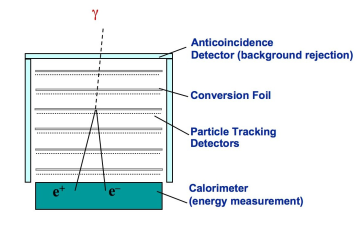
\includegraphics[width=0.451\textwidth]{figs/lat.png}
\caption{Cross-section of LAT}
\end{center}
\end{figure}


\subsection{Gamma ray spirals in a helical magnetic field}
Assume a position located within the particle jet opening angle of a blazar but are off-axis.  A photon of energy $E1 \sim 1TeV$ from the blazar propagates a distance, $D_{E1} \sim 100 Mpc$ and then scatters with an extragalactic background light photon to produce an electron-positron pair [cite 1,14]. As the electron positron trajectories are bent due to the Lorentz force by a magnetic field, the GeV photon cascade carries information about the structure of the cosmological magnetic field and, after a typical distance of about 30 kpc, up-scatters, via inverse Compton scattering, a cosmic microwave background photon, that arrives to an observer at the vectorial position denoted by $\vartheta_{1}$, which lies on the observer plane. At the same time another photon, with energy $E_{2}$, arrives at a second vectorial position, $\vartheta_{2}$ in the same plane. \cite{2} \cite{4}
The $\vartheta$ term can be expressed as: 
\begin{equation}
\vartheta \equiv \frac{\delta x_{i}-\delta x_{f} }{D_e}
\end{equation}
Where: 
\begin{itemize}
\item $\delta x_{f}$ is $\delta x(t) at t = t_{f},$ final time, i.e. when the particle up-scatters, $\delta x(t)$ is the position deviations induced by the magnetic field \cite{4}
\item $D_{e}$ is the distance traveled.
\end{itemize}
This can be shown in \cref{De}. 
\begin{figure}[hbt!] \label{De}
\begin{center}
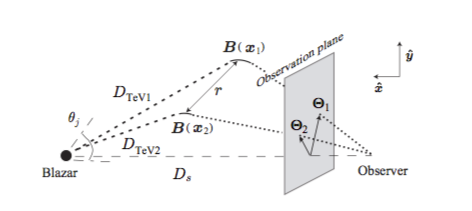
\includegraphics[width=0.451\textwidth]{figs/b.png}
\caption{Events at two different energies sample the magnetic field in regions of a certain size, $D_{e}$ \cite{4}}
\end{center}
\end{figure}
Working through the mathematics, which is done out fully in \cite{4}, an approximation of the position of the blazar using the position of the highest energy photon and relevant correlator. The correlator in this case is is the helical correlator, $G(E_{1}, E_{2})$, as this is a measure of CP violation\cite{18}:
\begin{equation} 
G(E_{1}, E_{2}) = \left \langle {\vartheta (E_{1}) \wedge \vartheta (E_{2}) \cdot \hat{x}} \right \rangle
\end{equation}
Where: 
\begin{itemize} 
\item $\hat{x}$ is perpendicular to the plane of observation and points in the direction of te source. 
\item The correlator is defined only if the blazar is visible, detectable, as the vectors $\vartheta_{1}, \vartheta_{2}$ originate at the line of sight intersects the observational plane. \cite{4}
\end{itemize}
However, diffuse gamma rays are observed on a sphere, i.e. the sky, and not on a plane and so the statistic $G(E1,E2;E3)$ needs to be modified in accordance to this, so the statistic becomes: 
\begin{equation}
Q'(E_{1}, E_{2}, E_{3}) = \left \langle {({n}(E_{1}))-{n}(E_{3})\wedge({n}(E_{2}-{n}(E_{3})\cdot {E_{3}}) } \right \rangle = \left \langle {{n}(E_{1}) \wedge {n}(E_{2})\cdot {n}(E_{3})} \right \rangle
\end{equation}
Where, $n(E)$ denotes the unit vector to the location of the photon with energy, E, on the sky. the highest energy E3 photons approximately represent the source directions. Lower energy (E1 and E2) photons in patches of some radius R around the position of the E3 photon are more likely to be from the same source \cite{2}.
See \cref{sky} for illustration, showing that gamma rays distributed on the sky. This figure demonstrates whether the directed curves from E3 to E2 to E1 are bent to the left or to the right, i.e. are the photons of decreasing energy in patterns of left-handed or right-handed spirals? A positive value of the statistic Q implies that there is an excess of right-handed spirals in the gamma ray sky and a negative value implies a left-handed excess.\cite{2}
\begin{figure}[hbt!] \label{sky}
\begin{center}
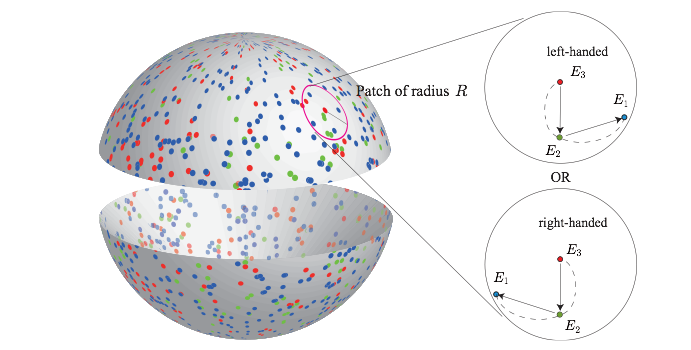
\includegraphics[width=0.451\textwidth]{figs/s.png}
\caption{Events at two different energies sample the magnetic field  in regions of a certain size, $D_{e} \cite{2}$}
\end{center}
\end{figure}
The final expression, which can be see \cite{2}\cite{4}, becomes:
\begin{equation}
Q(E_{1}, E_{2}, E_{3}, R) = \frac{1}{N_{1}N_{2}N_{3}}\sum_{i=1}^{N-{1}}\sum_{j=1}^{N-{2}}\sum_{k=1}^{N-{3}}W_{R}(n_{i}(E_{1}) \cdot n_{k}(E_{3})) W_{R}(n_{j}(E_{2}) \cdot n_{k}(E_{3})) n_{i}(E_{1}) \wedge n_{j}(E_{2}) \cdot n_{k}(E_{3})
\end{equation}
Where the indices refer to the different photons and $W_{R}$ is a top hat window function.
\begin{equation}
W_{R}(cos\alpha) = \left \{\begin{matrix}
1 & for~~ \alpha \leq ~ R \\ 
0, & otherwise
\end{matrix}\right.
\end{equation}

\subsection{Evaluation of the theory}
The above processes, though theoretically sound, possess certain difficulties in proving experimentally. The mathematics assume, for it to work, that the electron-position pair interact with the cosmological magnetic field, which is helical in nature.\cite{6} \cite{3} However, it would not be until the strength of the field was determined, it would not be known if the bending of the particle's trajectory is due to the magnetic field induced by the TeV blazar; who's magnetic field also exhibits a corkscrew field line pattern, due to its rotation. Recent gamma ray observations suggest the existence of cosmological magnetic fields of approximately $10^{-16}$ Gauss. \cite{6}
So in conclusion, again considering the below equation \cite{4}: 
\begin{equation}
h = \frac{1}{v} \int_{V} d^{3}x ~\vec{A} \cdot \vec{B}.
\end{equation}
Magnetic helicity is odd under CP transformations as A and B are odd under C-symmetry , while A is even but B is odd under P, parity \cite{18}. Non-zero magnetic helicity is predicted in scenarios in which cosmic baryogenesis and magnetogenesis occur concurrently during a cosmological phase transition, the electro-weak. Then the magnetic helicity density is related to the cosmic baryon number density and the CP violation responsible for the excess of matter over antimatter also provides helicity to the magnetic field. \cite{18}\cite{2} \cite{4}


%\
%~\\
%~\\
%~\\





%~\\
%~\\
%~\\
%~\\






%\end{document}
